\documentclass[11pt,a4paper]{article}
\usepackage[utf8]{inputenc}
\usepackage[T1]{fontenc}
\usepackage[spanish,es-tabla]{babel}
\usepackage{amsmath,amssymb}
\usepackage{graphicx}
\usepackage{booktabs}
\usepackage{geometry}
\usepackage{float}
\usepackage{hyperref}
\usepackage{cite}

\geometry{margin=2.4cm}
\hypersetup{colorlinks=true, linkcolor=blue, citecolor=blue, urlcolor=blue}

% Busca las figuras tanto en la carpeta actual (Overleaf) como en ../figures/ (Repositorio Git)
\graphicspath{{./}{../figures/}{figures/}}

\title{\vspace{-1.2cm}\textbf{Nota Técnica Hito 1: Evaluación Reproducible de la Respuesta Carga-Deflexión en una Viga Simplemente Apoyada}}
\author{Luis Angel Broncano Marcelo \\ \small Ingeniería Civil en Obras Civiles, Universidad de Santiago de Chile (USACH)}
\date{5 de octubre de 2026}

\begin{document}

\maketitle

\section{Definición del Problema y Objetivo}
El análisis de deformaciones en elementos sometidos a flexión constituye un requisito fundamental para verificar los estados límite de servicio en estructuras de ingeniería civil. El presente estudio aborda el caso de una viga prismática de sección rectangular ($b \times h$), simplemente apoyada en sus extremos $A$ y $B$ con una luz libre $L$, sometida a la acción de una carga puntual centrada $P$, tal como se ilustra en la Figura \ref{fig:esquema}.

\begin{figure}[H]
    \centering
    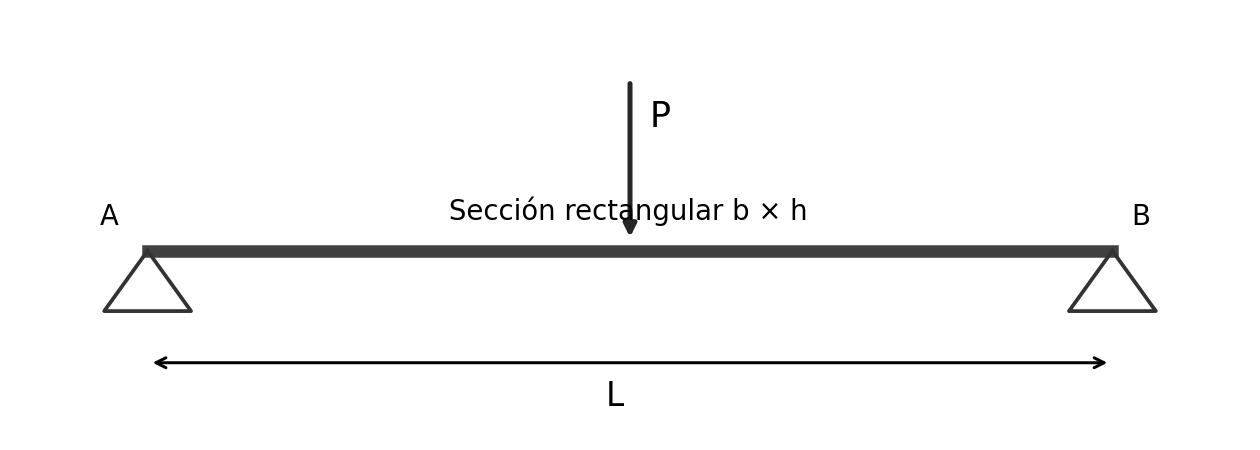
\includegraphics[width=0.68\textwidth]{esquema_viga.png}
    \caption{Esquema estructural de la viga simplemente apoyada con carga puntual centrada $P$.}
    \label{fig:esquema}
\end{figure}

El objetivo de esta nota técnica es implementar un flujo de trabajo computacional completamente trazable y reproducible para contrastar un conjunto de mediciones sintéticas de carga-deflexión en el centro de la luz ($\delta_{\text{med}}$) frente a la predicción analítica lineal elástica de la teoría clásica de vigas de Euler-Bernoulli ($\delta_{\text{teo}}$), evaluando su discrepancia relativa, verificando la consistencia física del modelo e identificando sus limitaciones mecánicas.

\section{Datos de Entrada, Supuestos y Metodología}

\subsection{Parámetros Geométricos, Materiales y Conversión de Unidades}
Los archivos originales de entrada (\texttt{datos\_viga.csv} y \texttt{parametros\_viga.xlsx}) se preservaron sin modificaciones en el directorio \texttt{data/} del repositorio. Para evitar errores de escala durante el procesamiento algebraico en la planilla \texttt{analysis/analisis\_viga.xlsx}, todas las magnitudes se transformaron de forma explícita al sistema consistente de unidades $(\text{N}, \text{mm})$, según se detalla en la Tabla \ref{tab:parametros}.

\begin{table}[H]
\centering
\caption{Parámetros del caso de estudio y factores de conversión al sistema consistente $(\text{N}, \text{mm})$.}
\label{tab:parametros}
\begin{tabular}{@{}llccll@{}}
\toprule
\textbf{Parámetro} & \textbf{Descripción} & \textbf{Valor Orig.} & \textbf{Unidad} & \textbf{Factor de Conversión} & \textbf{Valor Convertido} \\ \midrule
$L$ & Luz entre apoyos & $4.0$ & $\text{m}$ & $\times 10^{3}\text{ mm/m}$ & $4000\text{ mm}$ \\
$b$ & Ancho de la sección & $0.2$ & $\text{m}$ & $\times 10^{3}\text{ mm/m}$ & $200\text{ mm}$ \\
$h$ & Altura de la sección & $0.4$ & $\text{m}$ & $\times 10^{3}\text{ mm/m}$ & $400\text{ mm}$ \\
$E$ & Módulo de elasticidad & $25.0$ & $\text{GPa}$ & $\times 10^{3}\text{ (N/mm}^2\text{)/GPa}$ & $25\,000\text{ N/mm}^2$ \\
$P$ & Carga puntual aplicada & $0 \text{ a } 40$ & $\text{kN}$ & $\times 10^{3}\text{ N/kN}$ & $0 \text{ a } 40\,000\text{ N}$ \\ \bottomrule
\end{tabular}
\end{table}

\subsection{Formulación Teórica y Supuestos Mecánicos}
De acuerdo con la teoría clásica de flexión de Euler-Bernoulli \cite{hibbeler2017mecanica, gere2013mecanica}, el segundo momento de área centroidal $I$ para una sección transversal rectangular de base $b$ y altura $h$ respecto a su eje neutro horizontal viene dado por:
\begin{equation}
    I = \frac{b \cdot h^3}{12} = \frac{200\text{ mm} \cdot (400\text{ mm})^3}{12} = 1\,066\,666\,666.67\text{ mm}^4 \approx 1.0667 \times 10^{-3}\text{ m}^4
    \label{eq:inercia}
\end{equation}

La deflexión vertical máxima en el centro de la luz ($\delta_{\text{teo}}$) para una viga simplemente apoyada bajo carga puntual centrada $P$ se obtiene integrando la ecuación diferencial de la elástica ($E I \, d^2v/dx^2 = M(x)$):
\begin{equation}
    \delta_{\text{teo}} = \frac{P \cdot L^3}{48 \cdot E \cdot I}
    \label{eq:deflexion}
\end{equation}

Esta expresión descansa sobre cuatro supuestos fundamentales \cite{gere2013mecanica}: (1) el material es continuo, homogéneo, isotrópico y obedece la ley de Hooke (elasticidad lineal); (2) la viga experimenta pequeñas deformaciones y rotaciones ($dv/dx \ll 1$); (3) las secciones planas perpendiculares al eje longitudinal antes de la deformación permanecen planas y perpendiculares al eje deformado (despreciando la deformación angular por esfuerzo cortante); y (4) los apoyos son idealmente rígidos en dirección vertical y libres de fricción rotacional.

Para cuantificar la discrepancia entre las mediciones sintéticas ($\delta_{\text{med}}$) y el modelo analítico ($\delta_{\text{teo}}$) en el dominio $P > 0$, se define la diferencia relativa porcentual $\varepsilon_r$ como:
\begin{equation}
    \varepsilon_r (\%) = \frac{|\delta_{\text{med}} - \delta_{\text{teo}}|}{\delta_{\text{teo}}} \times 100
    \label{eq:error}
\end{equation}

\section{Resultados y Verificación del Modelo}

La Tabla \ref{tab:resultados} presenta los resultados obtenidos en \texttt{analysis/analisis\_viga.xlsx} para los nueve escalones de carga, incluyendo la razón de flexibilidad experimental $\delta_{\text{med}}/P$ y teórica $\delta_{\text{teo}}/P$. Asimismo, la Figura \ref{fig:comparacion} ilustra gráficamente el ajuste entre ambas series.

\begin{table}[H]
\centering
\caption{Comparación entre deflexión medida y predicción teórica de Euler-Bernoulli.}
\label{tab:resultados}
\begin{tabular}{@{}ccccccc@{}}
\toprule
$P$ ($\text{kN}$) & $P$ ($\text{N}$) & $\delta_{\text{med}}$ ($\text{mm}$) & $\delta_{\text{teo}}$ ($\text{mm}$) & $\delta_{\text{med}} - \delta_{\text{teo}}$ ($\text{mm}$) & $\varepsilon_r$ ($\%$) & $\delta_{\text{med}}/P$ ($\text{mm/kN}$) \\ \midrule
$0$  & $0$       & $0.00$ & $0.00$ & $0.00$  & ---    & ---     \\
$5$  & $5\,000$  & $0.26$ & $0.25$ & $+0.01$ & $4.00$ & $0.05200$ \\
$10$ & $10\,000$ & $0.50$ & $0.50$ & $0.00$  & $0.00$ & $0.05000$ \\
$15$ & $15\,000$ & $0.76$ & $0.75$ & $+0.01$ & $1.33$ & $0.05067$ \\
$20$ & $20\,000$ & $1.01$ & $1.00$ & $+0.01$ & $1.00$ & $0.05050$ \\
$25$ & $25\,000$ & $1.28$ & $1.25$ & $+0.03$ & $2.40$ & $0.05120$ \\
$30$ & $30\,000$ & $1.54$ & $1.50$ & $+0.04$ & $2.67$ & $0.05133$ \\
$35$ & $35\,000$ & $1.77$ & $1.75$ & $+0.02$ & $1.14$ & $0.05057$ \\
$40$ & $40\,000$ & $2.05$ & $2.00$ & $+0.05$ & $2.50$ & $0.05125$ \\ \bottomrule
\end{tabular}
\end{table}

\begin{figure}[H]
    \centering
    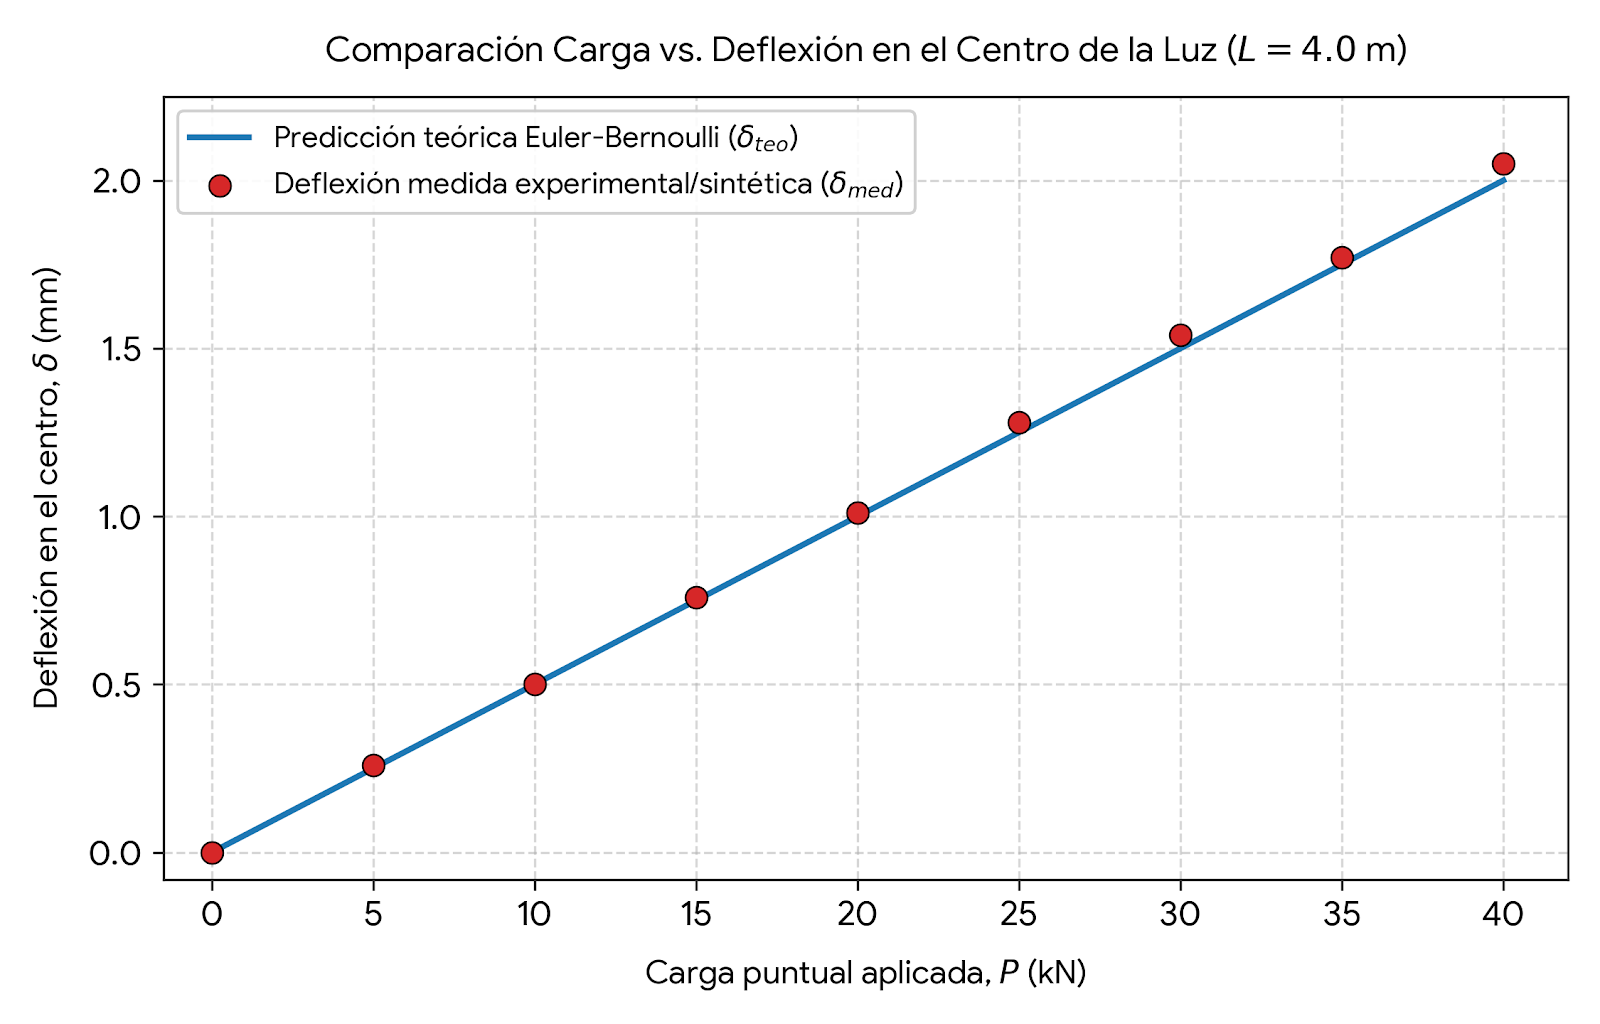
\includegraphics[width=0.78\textwidth]{carga_deflexion.png}
    \caption{Curva carga-deflexión comparativa entre los datos medidos y el modelo lineal de Euler-Bernoulli.}
    \label{fig:comparacion}
\end{figure}

Con el propósito de garantizar la confiabilidad de los resultados numéricos, se ejecutaron tres procedimientos de verificación independientes:
\begin{enumerate}
    \item \textbf{Verificación de homogeneidad dimensional:} Al sustituir las unidades consistentes en la Ecuación (\ref{eq:deflexion}), se comprueba que el resultado entrega unidades de longitud pura:
    \[
        [\delta_{\text{teo}}] = \frac{[\text{N}] \cdot [\text{mm}]^3}{[\text{N/mm}^2] \cdot [\text{mm}]^4} = \frac{[\text{N}] \cdot [\text{mm}]^3}{[\text{N}] \cdot [\text{mm}]^2} = [\text{mm}]
    \]
    \item \textbf{Comprobación manual de una fila de cálculo:} Evaluando de forma independiente el escalón intermedio $P = 20\text{ kN} = 20\,000\text{ N}$ (fila 5 de la Tabla \ref{tab:resultados}):
    \[
        \delta_{\text{teo}}(20\text{ kN}) = \frac{20\,000\text{ N} \cdot (4000\text{ mm})^3}{48 \cdot 25\,000\text{ N/mm}^2 \cdot 1.06667 \times 10^9\text{ mm}^4} = \frac{1.28 \times 10^{15}\text{ N}\cdot\text{mm}^3}{1.28 \times 10^{15}\text{ N}\cdot\text{mm}^2} = 1.00\text{ mm}
    \]
    El valor coincide exactamente con el reportado en la planilla, descartando errores de referencia celular.
    \item \textbf{Constancia de la flexibilidad ($\delta/P$) en el rango lineal:} La flexibilidad teórica de la viga es constante e igual a $f_{\text{teo}} = \delta_{\text{teo}}/P = 0.05000\text{ mm/kN}$ (equivalente a una rigidez flexional $K = 48EI/L^3 = 20\text{ kN/mm}$). En los datos medidos, la razón $\delta_{\text{med}}/P$ presenta un promedio de $0.05094\text{ mm/kN}$ con una desviación estándar de apenas $0.00062\text{ mm/kN}$ ($\text{CV} = 1.22\%$), confirmando que el sistema responde dentro de un régimen globalmente lineal.
\end{enumerate}

\section{Interpretación, Limitaciones y Conclusiones}

El análisis estadístico de las diferencias relativas para $P > 0$ muestra una discrepancia media de $1.88\%$ (mediana de $1.87\%$), oscilando entre un mínimo de $0.00\%$ para $P = 10\text{ kN}$ y un máximo de $4.00\%$ para $P = 5\text{ kN}$. El valor máximo porcentual en $P = 5\text{ kN}$ se explica por el efecto de resolución o redondeo a dos decimales ($0.01\text{ mm}$ de diferencia sobre una magnitud pequeña de $0.25\text{ mm}$). No obstante, una inspección crítica de la Tabla \ref{tab:resultados} revela un sesgo físico sistemático: en todos los niveles de carga no nulos se cumple que $\delta_{\text{med}} \ge \delta_{\text{teo}}$, con diferencias positivas que alcanzan $+0.05\text{ mm}$ a los $40\text{ kN}$.

Esta subestimación sistemática por parte del modelo de Euler-Bernoulli pone de manifiesto dos limitaciones principales:
\begin{itemize}
    \item \textbf{Omisión de la deformación por corte (Teoría de Timoshenko):} La viga analizada posee una relación de esbeltez moderada ($L/h = 4.0\text{ m} / 0.4\text{ m} = 10$). Al considerar la flexibilidad adicional por cortante $\delta_{\text{corte}} = P L / (4 G A_s)$ \cite{gere2013mecanica} ---asumiendo un coeficiente de Poisson típico de $\nu = 0.20$ para hormigón ($E = 25\text{ GPa} \Rightarrow G = 10.42\text{ GPa}$) y un área efectiva de corte $A_s = \frac{5}{6}bh = 0.0667\text{ m}^2$---, la flexibilidad adicional por corte resulta ser de $0.00144\text{ mm/kN}$. Al sumarla a la flexibilidad de flexión ($0.05000\text{ mm/kN}$), se obtiene una flexibilidad total de Timoshenko de $0.05144\text{ mm/kN}$ (lo que predice $\delta = 2.06\text{ mm}$ para $P = 40\text{ kN}$), explicando con notable exactitud el exceso observado en los datos sintéticos ($\bar{f}_{\text{med}} = 0.05094\text{ mm/kN}$ y $\delta_{\text{med}}(40\text{ kN}) = 2.05\text{ mm}$).
    \item \textbf{Idealización del material y de las condiciones de borde:} El modelo elástico lineal ignora la posible fisuración por tracción (en caso de tratarse de una sección de hormigón con $E = 25\text{ GPa}$) y asume apoyos infinitamente rígidos, donde cualquier micro-asentamiento incrementa la lectura de deflexión.
\end{itemize}

En conclusión, el modelo de Euler-Bernoulli reproduce satisfactoriamente el comportamiento global carga-deflexión de la viga con un error relativo promedio inferior al $2\%$. Sin embargo, la evidencia demuestra que las mediciones superan sistemáticamente la predicción clásica en alrededor de un $1.9\%$, fenómeno consistente con la contribución de las deformaciones por esfuerzo cortante en vigas de relación $L/h = 10$ y la precisión instrumental de $0.01\text{ mm}$. Finalmente, la estructuración modular del repositorio garantiza que cada resultado gráfico y numérico sea íntegramente auditable y reproducible desde los datos primarios.

\section*{Declaración de Uso de Inteligencia Artificial}
En conformidad con los lineamientos de integridad académica del curso, se declara el uso de la herramienta de inteligencia artificial generativa \textbf{Google Gemini} como asistente de apoyo durante el desarrollo de esta evaluación. El propósito de su uso se circunscribió a la estructuración del flujo de trabajo en Git, la revisión de formato tipográfico en \LaTeX{} y la contrastación de la hipótesis de deformación por cortante. Todo cálculo de inercia, conversión de unidades, formulación en planilla Excel y verificación numérica fue comprobado de manera independiente mediante cálculo manual y análisis dimensional, asumiendo el autor la responsabilidad total sobre la validez y defensa técnica del documento entregado (el registro detallado se encuentra en el archivo \texttt{USO\_IA.md} en la raíz del repositorio).

\bibliographystyle{plain}
\bibliography{referencias}

\end{document}